\documentclass[11pt]{article}

\usepackage[T1]{fontenc}
\usepackage[utf8]{inputenc}
\usepackage{lmodern}
\usepackage{microtype}
\usepackage[margin=0.82in]{geometry}
\usepackage{amsmath,amssymb,mathtools}
\usepackage{booktabs}
\usepackage{array}
\usepackage{enumitem}
\usepackage[most]{tcolorbox}
\usepackage{tikz}
\usetikzlibrary{arrows.meta,calc,decorations.pathreplacing,positioning}
\usepackage{fancyhdr}
\usepackage{hyperref}
\usepackage{needspace}
\usepackage{graphicx}
\usepackage{multicol}

\hypersetup{
  colorlinks=true,
  linkcolor=blue!55!black,
  urlcolor=blue!55!black,
  pdftitle={Exercise 9.10: The Historical Holder Inequality},
  pdfauthor={OpenAI}
}

\setlength{\parindent}{0pt}
\setlength{\parskip}{0.62em}
\setlist[itemize]{leftmargin=1.55em,itemsep=0.25em,topsep=0.25em}
\setlist[enumerate]{leftmargin=1.8em,itemsep=0.35em,topsep=0.3em}
\allowdisplaybreaks
\setcounter{tocdepth}{1}

\pagestyle{fancy}
\fancyhf{}
\lhead{Exercise 9.10 Tutorial}
\rhead{Historical H\"older Inequality}
\cfoot{\thepage}
\setlength{\headheight}{14pt}

\definecolor{navy}{RGB}{24,55,93}
\definecolor{softblue}{RGB}{235,244,252}
\definecolor{softgreen}{RGB}{236,248,239}
\definecolor{softyellow}{RGB}{255,249,226}
\definecolor{softred}{RGB}{253,239,239}
\definecolor{softgray}{RGB}{245,246,248}
\definecolor{softpurple}{RGB}{245,239,251}

\newtcolorbox{problemBox}{
  enhanced,
  colback=softblue,
  colframe=navy,
  boxrule=0.8pt,
  arc=2mm,
  title=The problem,
  fonttitle=\bfseries,
  breakable
}

\newtcolorbox{ideaBox}[1][Key idea]{
  enhanced,
  colback=softgreen,
  colframe=green!45!black,
  boxrule=0.7pt,
  arc=2mm,
  title={#1},
  fonttitle=\bfseries,
  breakable
}

\newtcolorbox{warningBox}[1][Watch out]{
  enhanced,
  colback=softyellow,
  colframe=orange!65!black,
  boxrule=0.7pt,
  arc=2mm,
  title={#1},
  fonttitle=\bfseries,
  breakable
}

\newtcolorbox{solutionBox}[1][Solution step]{
  enhanced,
  colback=white,
  colframe=navy!75,
  boxrule=0.8pt,
  arc=2mm,
  title={#1},
  fonttitle=\bfseries,
  breakable
}

\newtcolorbox{definitionBox}[1][Definition]{
  enhanced,
  colback=softgray,
  colframe=black!45,
  boxrule=0.6pt,
  arc=2mm,
  title={#1},
  fonttitle=\bfseries,
  breakable
}

\newtcolorbox{extraBox}[1][Extra insight]{
  enhanced,
  colback=softpurple,
  colframe=purple!55!black,
  boxrule=0.7pt,
  arc=2mm,
  title={#1},
  fonttitle=\bfseries,
  breakable
}

\newcommand{\abs}[1]{\left|#1\right|}
\newcommand{\R}{\mathbb{R}}
\newcommand{\Hist}{\mathrm{Hist}}
\newcommand{\Mod}{\mathrm{Mod}}

\begin{document}

\begin{center}
  {\LARGE\bfseries Exercise 9.10: The Historical H\"older Inequality}\\[0.35em]
  {\Large How weighted Jensen and modern H\"older are the same idea in disguise}\\[0.7em]
  {\large A step-by-step tutorial for a high-school reader}
\end{center}

\vspace{0.4em}

\begin{ideaBox}[What you will learn]
By the end of this tutorial, you will be able to:
\begin{itemize}
  \item understand weights and weighted averages;
  \item recognize why the function \(t\mapsto t^p\) is convex for \(p>1\);
  \item apply weighted Jensen's inequality to prove H\"older's historical formula;
  \item understand conjugate exponents \(p,q\) satisfying \(1/p+1/q=1\);
  \item turn the modern H\"older inequality into the historical one by splitting a factor;
  \item reverse that substitution and recover the modern inequality;
  \item identify the equality condition in both forms.
\end{itemize}
\end{ideaBox}

\tableofcontents

\section{The exercise, stated carefully}

\begin{problemBox}
Let \(w_1,\ldots,w_n\geq0\), let \(y_1,\ldots,y_n\geq0\), and let \(p>1\). Prove from weighted Jensen's inequality that
\[
 \boxed{\displaystyle
 \sum_{k=1}^{n}w_ky_k
 \leq
 \left(\sum_{k=1}^{n}w_k\right)^{(p-1)/p}
 \left(\sum_{k=1}^{n}w_ky_k^p\right)^{1/p}.}
 \tag{H$_{\mathrm{hist}}$}
\]
Then show that this historical form is equivalent to the modern H\"older inequality. Namely, if \(p,q>1\) satisfy
\[
 \frac1p+\frac1q=1,
\]
show that \((\mathrm{H}_{\mathrm{hist}})\) and
\[
 \boxed{\displaystyle
 \sum_{k=1}^{n}a_kb_k
 \leq
 \left(\sum_{k=1}^{n}a_k^p\right)^{1/p}
 \left(\sum_{k=1}^{n}b_k^q\right)^{1/q}}
 \tag{H$_{\mathrm{modern}}$}
\]
imply one another for nonnegative sequences \((a_k)\) and \((b_k)\).
\end{problemBox}

\begin{warningBox}[What if the entries can be negative?]
The exercise assumes nonnegative numbers because real powers such as \(a_k^p\) may be undefined when \(a_k<0\) and \(p\) is not an integer. For arbitrary real sequences, the standard form is
\[
 \abs{\sum_{k=1}^{n}a_kb_k}
 \leq
 \left(\sum_{k=1}^{n}\abs{a_k}^p\right)^{1/p}
 \left(\sum_{k=1}^{n}\abs{b_k}^q\right)^{1/q}.
\]
It follows from the nonnegative version by applying it to \(\abs{a_k}\) and \(\abs{b_k}\), then using
\[
 \abs{\sum a_kb_k}\leq\sum\abs{a_kb_k}.
\]
\end{warningBox}

\section{Background: the ideas used in the proof}

\subsection{Weights and weighted averages}

Suppose the numbers \(y_1,\ldots,y_n\) are measurements and the nonnegative numbers \(w_1,\ldots,w_n\) tell us how important each measurement is. Their total weight is
\[
 W:=\sum_{k=1}^{n}w_k.
 \tag{1}
\]
When \(W>0\), the weighted average is
\[
 \overline y_w
 :=\frac{w_1y_1+\cdots+w_ny_n}{w_1+\cdots+w_n}
 =\frac{\sum_{k=1}^{n}w_ky_k}{W}.
 \tag{2}
\]

For example, let \(y_1=2\), \(y_2=4\), with weights \(w_1=1\), \(w_2=3\). Then
\[
 \overline y_w=\frac{1\cdot2+3\cdot4}{1+3}=\frac{14}{4}=3.5.
\]
The answer is closer to \(4\) than to \(2\) because the value \(4\) has three times as much weight.

It is often convenient to normalize the weights:
\[
 \lambda_k:=\frac{w_k}{W}.
 \tag{3}
\]
Then
\[
 \lambda_k\geq0,
 \qquad
 \sum_{k=1}^{n}\lambda_k=1,
 \qquad
 \overline y_w=\sum_{k=1}^{n}\lambda_ky_k.
 \tag{4}
\]
Thus the \(\lambda_k\)'s are percentages written as decimals: they describe how the total weight is divided among the entries.

\subsection{Convex functions}

A convex function bends upward like a bowl. The important geometric fact is that the straight chord joining two points of its graph lies on or above the graph.

For this problem we use
\[
 f(t)=t^p,
 \qquad t\geq0,
 \qquad p>1.
 \tag{5}
\]
This function is convex. For example, when \(p=2\), its graph is the parabola \(f(t)=t^2\).

\begin{center}
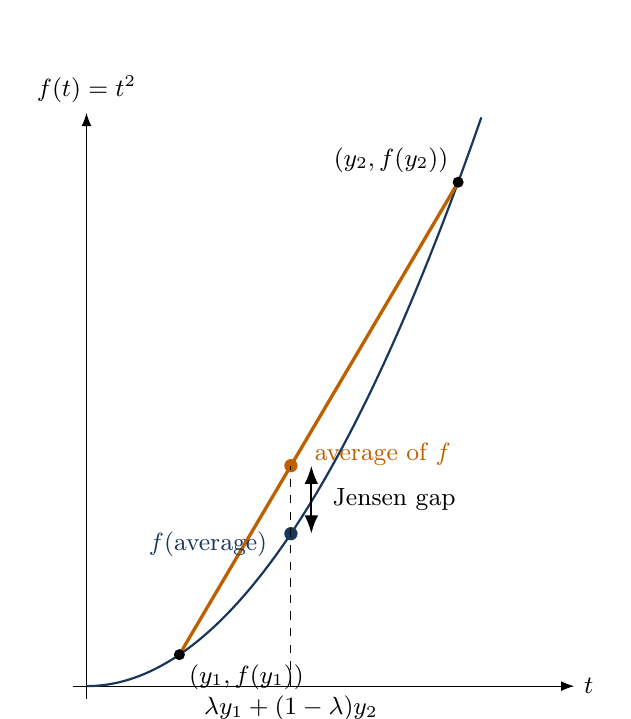
\begin{tikzpicture}[x=1.18cm,y=0.40cm,>=Latex,font=\small]
  \draw[->] (-0.15,0)--(5.25,0) node[right] {$t$};
  \draw[->] (0,-0.4)--(0,18.2) node[above] {$f(t)=t^2$};
  \draw[thick,navy,domain=0:4.25,samples=90] plot (\x,{\x*\x});

  \coordinate (A) at (1,1);
  \coordinate (B) at (4,16);
  \coordinate (Mcurve) at (2.2,4.84);
  \coordinate (Mchord) at (2.2,7);
  \draw[very thick,orange!75!black] (A)--(B);
  \fill (A) circle (2pt) node[below right] {$(y_1,f(y_1))$};
  \fill (B) circle (2pt) node[above left] {$(y_2,f(y_2))$};
  \fill[navy] (Mcurve) circle (2.4pt);
  \fill[orange!75!black] (Mchord) circle (2.4pt);
  \draw[dashed] (2.2,0)--(Mchord);
  \draw[<->,thick] (2.42,4.84)--(2.42,7)
    node[midway,right=4pt,align=left] {Jensen gap};
  \node[below] at (2.2,0) {$\lambda y_1+(1-\lambda)y_2$};
  \node[navy,anchor=east] at (2.05,4.5) {$f(\text{average})$};
  \node[orange!75!black,anchor=west] at (2.35,7.35) {$\text{average of }f$};
\end{tikzpicture}
\end{center}

The lower point is \(f\) evaluated at a weighted average of the inputs. The upper point is the same weighted average of the output heights. Convexity says the lower point cannot rise above the upper one.

\begin{extraBox}[Optional calculus check]
If you know derivatives, then for \(t>0\),
\[
 f''(t)=p(p-1)t^{p-2}\geq0.
\]
A nonnegative second derivative means the graph bends upward. Continuity at \(t=0\) extends convexity to all of \([0,\infty)\).
\end{extraBox}

\subsection{Weighted Jensen's inequality}

\begin{definitionBox}[Weighted Jensen inequality]
Let \(f\) be convex, and let \(\lambda_k\geq0\) satisfy \(\sum_{k=1}^{n}\lambda_k=1\). Then
\[
 \boxed{\displaystyle
 f\left(\sum_{k=1}^{n}\lambda_kx_k\right)
 \leq
 \sum_{k=1}^{n}\lambda_kf(x_k).}
 \tag{J}
\]
\end{definitionBox}

In words:
\[
 \boxed{\text{function of the weighted average}
 \ \leq\ \text{weighted average of the function values}.}
\]
For our choice \(f(t)=t^p\), Jensen becomes
\[
 \left(\sum_{k=1}^{n}\lambda_ky_k\right)^p
 \leq
 \sum_{k=1}^{n}\lambda_ky_k^p.
 \tag{6}
\]
This single inequality is the engine of the first proof.

\subsection{Conjugate exponents}

\begin{definitionBox}[Conjugate exponents]
Numbers \(p,q>1\) are called conjugate exponents when
\[
 \frac1p+\frac1q=1.
 \tag{7}
\]
If \(p>1\) is given, its conjugate is
\[
 q=\frac{p}{p-1}.
 \tag{8}
\]
\end{definitionBox}

Some examples are
\[
\begin{array}{c|c|c}
 p & q & 1/p+1/q\\ \hline
 2 & 2 & 1/2+1/2=1\\[2pt]
 3 & 3/2 & 1/3+2/3=1\\[2pt]
 4 & 4/3 & 1/4+3/4=1
\end{array}
\]
Two identities will be used repeatedly:
\[
 \frac1q=1-\frac1p=\frac{p-1}{p},
 \tag{9}
\]
and
\[
 \frac{q}{p}=q-1=\frac1{p-1}.
 \tag{10}
\]
For instance, the first identity explains why the historical exponent \((p-1)/p\) is really \(1/q\).

\section{First goal: derive the historical inequality from Jensen}

We now prove
\[
 \sum_{k=1}^{n}w_ky_k
 \leq
 \left(\sum_{k=1}^{n}w_k\right)^{(p-1)/p}
 \left(\sum_{k=1}^{n}w_ky_k^p\right)^{1/p}.
 \tag{11}
\]

\begin{solutionBox}[Step 0: handle the all-zero weight case]
Let
\[
 W=\sum_{k=1}^{n}w_k.
\]
If \(W=0\), then every \(w_k=0\), because the weights are nonnegative. Both sides of (11) are then \(0\), so the inequality is true.

From now on, assume \(W>0\).
\end{solutionBox}

\begin{solutionBox}[Step 1: turn the weights into normalized weights]
Define
\[
 \lambda_k:=\frac{w_k}{W}.
 \tag{12}
\]
Then \(\lambda_k\geq0\) and
\[
 \sum_{k=1}^{n}\lambda_k
 =\frac{\sum_{k=1}^{n}w_k}{W}
 =\frac{W}{W}=1.
 \tag{13}
\]
Therefore the \(\lambda_k\)'s satisfy the hypotheses of weighted Jensen.
\end{solutionBox}

\begin{solutionBox}[Step 2: apply Jensen to \(f(t)=t^p\)]
Since \(p>1\), the function \(f(t)=t^p\) is convex on \([0,\infty)\). Jensen gives
\[
 \left(\sum_{k=1}^{n}\lambda_ky_k\right)^p
 \leq
 \sum_{k=1}^{n}\lambda_ky_k^p.
 \tag{14}
\]
Substitute \(\lambda_k=w_k/W\):
\[
 \left(\frac{\sum_{k=1}^{n}w_ky_k}{W}\right)^p
 \leq
 \frac{\sum_{k=1}^{n}w_ky_k^p}{W}.
 \tag{15}
\]
\end{solutionBox}

\begin{solutionBox}[Step 3: take the positive \(p\)-th root]
All quantities in (15) are nonnegative. The function \(t\mapsto t^{1/p}\) is increasing on \([0,\infty)\), so taking the \(p\)-th root preserves the inequality:
\[
 \frac{\sum_{k=1}^{n}w_ky_k}{W}
 \leq
 \left(\frac{\sum_{k=1}^{n}w_ky_k^p}{W}\right)^{1/p}.
 \tag{16}
\]
\end{solutionBox}

\begin{solutionBox}[Step 4: multiply by \(W\) and simplify]
Multiplying (16) by \(W>0\) gives
\[
 \sum_{k=1}^{n}w_ky_k
 \leq
 W\left(\frac{\sum_{k=1}^{n}w_ky_k^p}{W}\right)^{1/p}.
 \tag{17}
\]
Now separate the power of \(W\):
\[
\begin{aligned}
 W\left(\frac{\sum w_ky_k^p}{W}\right)^{1/p}
 &=W\cdot W^{-1/p}\left(\sum w_ky_k^p\right)^{1/p}\\
 &=W^{1-1/p}\left(\sum w_ky_k^p\right)^{1/p}\\
 &=W^{(p-1)/p}\left(\sum w_ky_k^p\right)^{1/p}.
\end{aligned}
 \tag{18}
\]
Because \(W=\sum w_k\), this is exactly
\[
 \boxed{\displaystyle
 \sum_{k=1}^{n}w_ky_k
 \leq
 \left(\sum_{k=1}^{n}w_k\right)^{(p-1)/p}
 \left(\sum_{k=1}^{n}w_ky_k^p\right)^{1/p}.}
\]
\end{solutionBox}

\begin{ideaBox}[The proof in one line]
For \(W=\sum w_k>0\), weighted Jensen says
\[
 \left(\frac{\sum w_ky_k}{W}\right)^p
 \leq
 \frac{\sum w_ky_k^p}{W}.
\]
Taking the \(p\)-th root and multiplying by \(W\) gives the historical H\"older inequality.
\end{ideaBox}

\subsection{A numerical example}

Take
\[
 p=2,
 \qquad
 (w_1,w_2)=(1,3),
 \qquad
 (y_1,y_2)=(2,4).
\]
The left side is
\[
 \sum w_ky_k=1\cdot2+3\cdot4=14.
\]
The right side is
\[
 \left(1+3\right)^{1/2}
 \left(1\cdot2^2+3\cdot4^2\right)^{1/2}
 =2\sqrt{52}\approx14.422.
\]
Thus
\[
 14\leq14.422.
\]
In normalized Jensen form, the same calculation is
\[
 \left(\frac{14}{4}\right)^2=3.5^2=12.25
 \leq
 \frac{52}{4}=13.
\]
The historical inequality is therefore just this Jensen comparison rewritten without fractions.

\section{The factor-splitting picture}

The equivalence with modern H\"older becomes much easier when we notice the following exact factorization. Let \(q\) be conjugate to \(p\). Since \(1/p+1/q=1\),
\[
 w_ky_k
 =w_k^{1/p}w_k^{1/q}y_k
 =\left(w_k^{1/p}y_k\right)\left(w_k^{1/q}\right).
 \tag{19}
\]

\begin{center}
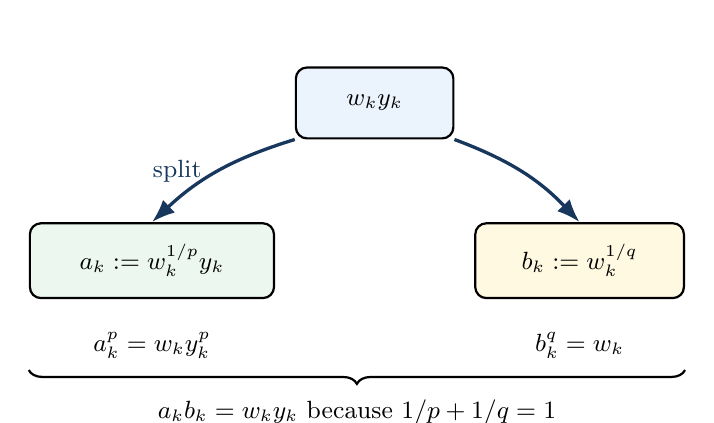
\begin{tikzpicture}[>=Latex,node distance=0.65cm and 0.75cm,font=\small]
  \node[draw,rounded corners,thick,fill=softblue,minimum width=2.0cm,minimum height=0.9cm] (whole)
    {$w_ky_k$};
  \node[draw,rounded corners,thick,fill=softgreen,below left=1.05cm and 0.25cm of whole,
    minimum width=3.1cm,minimum height=0.95cm] (left)
    {$a_k:=w_k^{1/p}y_k$};
  \node[draw,rounded corners,thick,fill=softyellow,below right=1.05cm and 0.25cm of whole,
    minimum width=2.65cm,minimum height=0.95cm] (right)
    {$b_k:=w_k^{1/q}$};
  \draw[->,very thick,navy] (whole.south west) to[bend right=13] node[left=2pt] {split} (left.north);
  \draw[->,very thick,navy] (whole.south east) to[bend left=13] (right.north);
  \node[below=0.30cm of left] {$a_k^p=w_ky_k^p$};
  \node[below=0.30cm of right] {$b_k^q=w_k$};
  \draw[decorate,decoration={brace,amplitude=5pt,mirror},thick]
    ($(left.south west)+(0,-0.9)$)--($(right.south east)+(0,-0.9)$)
    node[midway,below=7pt] {$a_kb_k=w_ky_k$ because $1/p+1/q=1$};
\end{tikzpicture}
\end{center}

This diagram already contains the proof that modern H\"older implies the historical version: apply modern H\"older to the two pieces.

\section{Modern H\"older implies the historical form}

Assume the modern H\"older inequality is known. Let \(p>1\), and define its conjugate exponent
\[
 q:=\frac{p}{p-1}.
 \tag{20}
\]
Then \(1/p+1/q=1\) and \(1/q=(p-1)/p\).

\begin{solutionBox}[Step 1: split each term \(w_ky_k\)]
Define two new sequences
\[
 a_k:=w_k^{1/p}y_k,
 \qquad
 b_k:=w_k^{1/q}.
 \tag{21}
\]
Then
\[
 a_kb_k=w_k^{1/p+1/q}y_k=w_ky_k.
 \tag{22}
\]
Also,
\[
 a_k^p=w_ky_k^p,
 \qquad
 b_k^q=w_k.
 \tag{23}
\]
\end{solutionBox}

\begin{solutionBox}[Step 2: apply modern H\"older]
Modern H\"older gives
\[
\begin{aligned}
 \sum_{k=1}^{n}w_ky_k
 &=\sum_{k=1}^{n}a_kb_k\\
 &\leq
 \left(\sum_{k=1}^{n}a_k^p\right)^{1/p}
 \left(\sum_{k=1}^{n}b_k^q\right)^{1/q}\\
 &=
 \left(\sum_{k=1}^{n}w_ky_k^p\right)^{1/p}
 \left(\sum_{k=1}^{n}w_k\right)^{1/q}.
\end{aligned}
 \tag{24}
\]
Finally, use \(1/q=(p-1)/p\):
\[
 \sum_{k=1}^{n}w_ky_k
 \leq
 \left(\sum_{k=1}^{n}w_k\right)^{(p-1)/p}
 \left(\sum_{k=1}^{n}w_ky_k^p\right)^{1/p}.
\]
This is the historical inequality.
\end{solutionBox}

\begin{ideaBox}[Why this direction is especially simple]
The weights are divided between the two modern H\"older factors:
\[
 w_k=w_k^{1/p}w_k^{1/q}.
\]
The \(y_k\) is placed entirely in the \(p\)-factor. Raising the first factor to the \(p\)-th power produces \(w_ky_k^p\), while raising the second to the \(q\)-th power produces \(w_k\).
\end{ideaBox}

\section{The historical form implies modern H\"older}

Now assume the historical inequality is known for every set of nonnegative weights and values. Let \(a_k,b_k\geq0\), and let \(p,q>1\) satisfy
\[
 \frac1p+\frac1q=1.
 \tag{25}
\]
We want to prove
\[
 \sum_{k=1}^{n}a_kb_k
 \leq
 \left(\sum_{k=1}^{n}a_k^p\right)^{1/p}
 \left(\sum_{k=1}^{n}b_k^q\right)^{1/q}.
 \tag{26}
\]

The idea is to reverse the factor split from the previous section. We want
\[
 a_k=w_k^{1/p}y_k,
 \qquad
 b_k=w_k^{1/q}.
 \tag{27}
\]
The second equation suggests
\[
 w_k=b_k^q.
 \tag{28}
\]
Then the first equation suggests
\[
 y_k=\frac{a_k}{w_k^{1/p}}
 =\frac{a_k}{b_k^{q/p}}.
 \tag{29}
\]

\begin{warningBox}[What about an index with \(b_k=0\)?]
Formula (29) would divide by zero. Such indices cause no real difficulty because \(a_kb_k=0\), so they contribute nothing to the left side. We may apply the argument only to the set
\[
 I:=\{k:b_k>0\}.
\]
Afterward, enlarging \(\sum_{k\in I}a_k^p\) to \(\sum_{k=1}^{n}a_k^p\) can only make the right side larger. If every \(b_k=0\), the desired inequality is simply \(0\leq0\).
\end{warningBox}

Assume therefore that \(I\) is nonempty, and for \(k\in I\) define
\[
 w_k:=b_k^q,
 \qquad
 y_k:=\frac{a_k}{b_k^{q/p}}.
 \tag{30}
\]

\begin{solutionBox}[Step 1: simplify the left side of the historical inequality]
For \(k\in I\),
\[
\begin{aligned}
 w_ky_k
 &=b_k^q\frac{a_k}{b_k^{q/p}}\\
 &=a_kb_k^{q-q/p}.
\end{aligned}
\]
Now
\[
 q-\frac{q}{p}
 =q\left(1-\frac1p\right)
 =q\left(\frac1q\right)
 =1.
 \tag{31}
\]
Therefore
\[
 w_ky_k=a_kb_k.
 \tag{32}
\]
\end{solutionBox}

\begin{solutionBox}[Step 2: simplify the powered sum]
Again for \(k\in I\),
\[
\begin{aligned}
 w_ky_k^p
 &=b_k^q\left(\frac{a_k}{b_k^{q/p}}\right)^p\\
 &=b_k^q\frac{a_k^p}{b_k^q}\\
 &=a_k^p.
\end{aligned}
 \tag{33}
\]
Also,
\[
 \sum_{k\in I}w_k=\sum_{k\in I}b_k^q=\sum_{k=1}^{n}b_k^q,
 \tag{34}
\]
because \(b_k^q=0\) outside \(I\).
\end{solutionBox}

\begin{solutionBox}[Step 3: apply the historical inequality]
Applying \((\mathrm{H}_{\mathrm{hist}})\) over \(I\) gives
\[
\begin{aligned}
 \sum_{k=1}^{n}a_kb_k
 &=\sum_{k\in I}w_ky_k\\
 &\leq
 \left(\sum_{k\in I}w_k\right)^{(p-1)/p}
 \left(\sum_{k\in I}w_ky_k^p\right)^{1/p}\\
 &=
 \left(\sum_{k=1}^{n}b_k^q\right)^{(p-1)/p}
 \left(\sum_{k\in I}a_k^p\right)^{1/p}\\
 &\leq
 \left(\sum_{k=1}^{n}b_k^q\right)^{1/q}
 \left(\sum_{k=1}^{n}a_k^p\right)^{1/p}.
\end{aligned}
 \tag{35}
\]
In the last line, we used \((p-1)/p=1/q\). Reordering the two factors gives the modern H\"older inequality.
\end{solutionBox}

\begin{ideaBox}[The reverse substitution]
To recover modern H\"older from the historical form, solve
\[
 a_k=w_k^{1/p}y_k,
 \qquad
 b_k=w_k^{1/q}.
\]
This leads to
\[
 \boxed{w_k=b_k^q,
 \qquad
 y_k=\frac{a_k}{b_k^{q/p}}.}
\]
That substitution is the main creative step. Everything afterward is exponent simplification.
\end{ideaBox}

\section{The complete equivalence loop}

The three inequalities fit together as follows.

\begin{center}
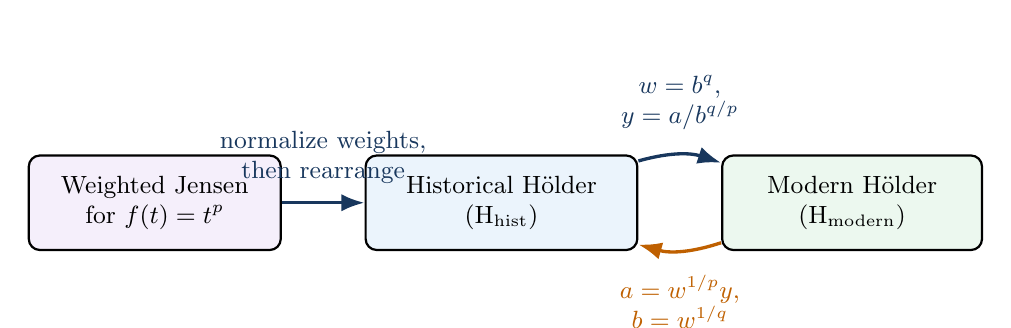
\begin{tikzpicture}[>=Latex,node distance=1.15cm and 1.05cm,font=\small]
  \node[draw,rounded corners,thick,fill=softpurple,align=center,minimum width=3.2cm,minimum height=1.2cm] (J)
    {Weighted Jensen\\for $f(t)=t^p$};
  \node[draw,rounded corners,thick,fill=softblue,align=center,right=of J,minimum width=3.45cm,minimum height=1.2cm] (H)
    {Historical H\"older\\$(\mathrm{H}_{\mathrm{hist}})$};
  \node[draw,rounded corners,thick,fill=softgreen,align=center,right=of H,minimum width=3.3cm,minimum height=1.2cm] (M)
    {Modern H\"older\\$(\mathrm{H}_{\mathrm{modern}})$};

  \draw[->,very thick,navy] (J)--(H)
    node[midway,above=3pt,align=center] {normalize weights,\\then rearrange};
  \draw[->,very thick,navy] (H) to[bend left=17] node[midway,above=5pt,align=center]
    {$w=b^q$,\\$y=a/b^{q/p}$} (M);
  \draw[->,very thick,orange!75!black] (M) to[bend left=17] node[midway,below=5pt,align=center]
    {$a=w^{1/p}y$,\\$b=w^{1/q}$} (H);
\end{tikzpicture}
\end{center}

Thus historical and modern H\"older are not merely similar. They are the same inequality written using different variables.

\section{Equality: when do the two sides match?}

The function \(t^p\) is strictly convex for \(p>1\). Therefore equality in weighted Jensen occurs precisely when all values \(y_k\) carrying positive weight are equal:
\[
 w_k>0\quad\Longrightarrow\quad y_k=c
 \tag{36}
\]
for some constant \(c\geq0\). This is also the equality condition in the historical inequality.

To translate it into the modern variables, use
\[
 w_k=b_k^q,
 \qquad
 y_k=\frac{a_k}{b_k^{q/p}}.
\]
Equality requires
\[
 \frac{a_k}{b_k^{q/p}}=c
 \qquad\text{whenever }b_k>0.
 \tag{37}
\]
Therefore
\[
 a_k=c\,b_k^{q/p}.
\]
Raising both sides to the \(p\)-th power gives
\[
 \boxed{a_k^p=c^p b_k^q.}
 \tag{38}
\]
So, apart from zero entries, equality in modern H\"older occurs when the powered sequences \((a_k^p)\) and \((b_k^q)\) are proportional.

\subsection{An equality example}

Take \(p=q=2\),
\[
 a=(1,2,3),
 \qquad
 b=(2,4,6)=2a.
\]
Then \(a_k^2=(1/4)b_k^2\), so the proportionality condition holds. Indeed,
\[
 \sum a_kb_k=2(1^2+2^2+3^2)=28,
\]
and
\[
 \left(\sum a_k^2\right)^{1/2}
 \left(\sum b_k^2\right)^{1/2}
 =\sqrt{14}\sqrt{56}=\sqrt{784}=28.
\]

\section{A second numerical example: seeing the two forms agree}

Let \(p=q=2\), and choose
\[
 w=(1,4),
 \qquad
 y=(3,2).
\]
The factor split gives
\[
 a_k=w_k^{1/2}y_k,
 \qquad
 b_k=w_k^{1/2}.
\]
Thus
\[
 a=(3,4),
 \qquad
 b=(1,2).
\]
The historical left side is
\[
 \sum w_ky_k=1\cdot3+4\cdot2=11,
\]
while the modern left side is the same number:
\[
 \sum a_kb_k=3\cdot1+4\cdot2=11.
\]
The historical right side is
\[
 (1+4)^{1/2}(1\cdot3^2+4\cdot2^2)^{1/2}
 =\sqrt5\sqrt{25}=5\sqrt5.
\]
The modern right side is also
\[
 \sqrt{3^2+4^2}\sqrt{1^2+2^2}
 =5\sqrt5.
\]
The two formulas give literally the same numerical inequality:
\[
 11\leq5\sqrt5.
\]

\section{Common mistakes and how to avoid them}

\begin{warningBox}[Mistake 1: forgetting the case \(\sum w_k=0\)]
Normalized weights \(w_k/W\) make sense only when \(W>0\). Check \(W=0\) first. Because the weights are nonnegative, \(W=0\) means every weight is zero, and the result is immediate.
\end{warningBox}

\begin{warningBox}[Mistake 2: applying Jensen to the wrong function]
The needed choice is
\[
 f(t)=t^p.
\]
Jensen then produces \(y_k^p\), exactly the power appearing in the historical inequality. Choosing \(f(t)=t^{1/p}\) would use a concave function and reverse the direction.
\end{warningBox}

\begin{warningBox}[Mistake 3: losing the factor \(W^{(p-1)/p}\)]
From
\[
 \frac{\sum w_ky_k}{W}
 \leq
 \left(\frac{\sum w_ky_k^p}{W}\right)^{1/p},
\]
multiplying by \(W\) gives
\[
 W\cdot W^{-1/p}=W^{1-1/p}=W^{(p-1)/p},
\]
not simply \(W\).
\end{warningBox}

\begin{warningBox}[Mistake 4: using \(w_k=b_k^p\) in the reverse direction]
To make the second modern norm equal \((\sum b_k^q)^{1/q}\), the correct choice is
\[
 w_k=b_k^q,
\]
not \(b_k^p\). The exponent \(q\) is forced by the equation \(b_k=w_k^{1/q}\).
\end{warningBox}

\begin{warningBox}[Mistake 5: dividing by \(b_k\) when \(b_k=0\)]
When reversing the substitution, restrict first to indices with \(b_k>0\). Terms with \(b_k=0\) contribute \(a_kb_k=0\) to the left side and can safely be omitted.
\end{warningBox}

\section{A compact solution suitable for homework}

\begin{solutionBox}[Concise proof]
Let \(W=\sum_{k=1}^{n}w_k\). If \(W=0\), the historical inequality is trivial. Assume \(W>0\), and set \(\lambda_k=w_k/W\). Since \(t\mapsto t^p\) is convex for \(p>1\), weighted Jensen gives
\[
 \left(\sum_{k=1}^{n}\lambda_ky_k\right)^p
 \leq
 \sum_{k=1}^{n}\lambda_ky_k^p.
\]
Hence
\[
 \left(\frac{\sum w_ky_k}{W}\right)^p
 \leq
 \frac{\sum w_ky_k^p}{W}.
\]
Taking the \(p\)-th root and multiplying by \(W\),
\[
 \sum w_ky_k
 \leq
 W^{1-1/p}\left(\sum w_ky_k^p\right)^{1/p}
 =W^{(p-1)/p}\left(\sum w_ky_k^p\right)^{1/p}.
\]
This proves the historical form.

Now let \(q=p/(p-1)\). If the modern inequality is assumed, apply it to
\[
 a_k=w_k^{1/p}y_k,
 \qquad
 b_k=w_k^{1/q}.
\]
Then \(a_kb_k=w_ky_k\), \(a_k^p=w_ky_k^p\), and \(b_k^q=w_k\), so modern H\"older becomes the historical inequality.

Conversely, assume the historical inequality. Given nonnegative \(a_k,b_k\), omit indices with \(b_k=0\), and put
\[
 w_k=b_k^q,
 \qquad
 y_k=\frac{a_k}{b_k^{q/p}}.
\]
Then
\[
 w_ky_k=a_kb_k,
 \qquad
 w_ky_k^p=a_k^p,
 \qquad
 \sum w_k=\sum b_k^q.
\]
The historical inequality therefore gives
\[
 \sum a_kb_k
 \leq
 \left(\sum b_k^q\right)^{(p-1)/p}
 \left(\sum a_k^p\right)^{1/p}
 =
 \left(\sum a_k^p\right)^{1/p}
 \left(\sum b_k^q\right)^{1/q},
\]
which is the modern H\"older inequality. Thus the two forms are equivalent.
\end{solutionBox}

\section{Self-check questions}

Try these before reading the answers.

\begin{enumerate}
  \item If \(p=3\), what is its conjugate exponent \(q\)?
  \item For \(p=4\), simplify \((p-1)/p\), and compare it with \(1/q\).
  \item Why does \(\sum w_k=0\) force every \(w_k=0\)?
  \item Starting from Jensen,
  \[
   \left(\frac{\sum w_ky_k}{W}\right)^p
   \leq
   \frac{\sum w_ky_k^p}{W},
  \]
  explain where the power \(W^{(p-1)/p}\) comes from.
  \item Verify that with
  \[
   a_k=w_k^{1/p}y_k,
   \qquad
   b_k=w_k^{1/q},
  \]
  one has \(a_k^p=w_ky_k^p\), \(b_k^q=w_k\), and \(a_kb_k=w_ky_k\).
  \item In the reverse substitution, why is \(w_k=b_k^q\) a natural choice?
  \item What is the equality condition in modern H\"older for positive entries?
\end{enumerate}

\begin{extraBox}[Answers]
\begin{enumerate}
  \item \(q=p/(p-1)=3/2\).
  \item \((p-1)/p=3/4\). The conjugate of \(4\) is \(q=4/3\), so \(1/q=3/4\).
  \item A sum of nonnegative numbers can equal zero only if every term is zero.
  \item Taking the \(p\)-th root produces a factor \(W^{-1/p}\) on the right. Multiplying both sides by \(W\) gives \(W\cdot W^{-1/p}=W^{1-1/p}=W^{(p-1)/p}\).
  \item Raise each definition to the matching power and use \(1/p+1/q=1\).
  \item We want \(b_k=w_k^{1/q}\). Raising both sides to the \(q\)-th power forces \(w_k=b_k^q\).
  \item There is a constant \(C\geq0\) such that \(a_k^p=C b_k^q\) for all relevant indices.
\end{enumerate}
\end{extraBox}

\section{Final summary}

\begin{ideaBox}[Three formulas to remember]
\small
Weighted Jensen with \(f(t)=t^p\) gives
\[
 \left(\frac{\sum w_ky_k}{\sum w_k}\right)^p
 \leq
 \frac{\sum w_ky_k^p}{\sum w_k}
 \quad\Longrightarrow\quad
 \sum w_ky_k
 \leq
 \left(\sum w_k\right)^{(p-1)/p}
 \left(\sum w_ky_k^p\right)^{1/p}.
\]
For conjugate \(p,q\), the two changes of variables are
\[
 \boxed{a_k=w_k^{1/p}y_k,\quad b_k=w_k^{1/q}}
 \qquad\text{and}\qquad
 \boxed{w_k=b_k^q,\quad y_k=\frac{a_k}{b_k^{q/p}}}\quad(b_k>0).
\]
They convert the historical and modern forms into one another.
\end{ideaBox}

\end{document}
